\documentclass{IEEEcsmag}

\usepackage[colorlinks,urlcolor=blue,linkcolor=blue,citecolor=blue]{hyperref}

\usepackage{xcolor}
\definecolor{bemppgrey}{HTML}{555555}
\definecolor{bempporange}{HTML}{FF7A1A}

\usepackage{pythonhighlight}

\usepackage{tikz}
\usetikzlibrary{arrows,decorations.pathreplacing}
\usepackage{ifthen}

\usepackage{upmath}
\usepackage{upgreek}
\usepackage{amsmath, amssymb}

\usepackage{cleveref}
\crefname{equation}{Equation}{Equations}
\Crefname{equation}{Equation}{Equations}
\crefname{figure}{Figure}{Figures}
\Crefname{figure}{Figure}{Figures}
\crefname{section}{Section}{Sections}
\Crefname{section}{Section}{Sections}

% Bold vector (for points in R^3)
\newcommand{\bvec}[1]{\boldsymbol{#1}}
\def\bx{\bvec{x}}
\def\by{\bvec{y}}
\newcommand{\ds}[1][]{\,\mathrm{d}s\ifthenelse{\equal{#1}{}}{}{_{#1}}}

% Discrete vector and discrete matrix
\newcommand{\dmat}[1]{\mathbf{#1}}
\newcommand{\dvec}[1]{\mathbf{#1}}

\newcommand{\ii}{\mathrm{i}}
\newcommand{\ee}{\mathrm{e}}


\jvol{XX}
\jnum{XX}
\paper{8}
\jmonth{May/June}
\jname{IT Professional}
\pubyear{2021}
\newtheorem{theorem}{Theorem}
\newtheorem{lemma}{Lemma}

\setcounter{secnumdepth}{0}

\begin{document}

\sptitle{Department: Head}
\editor{Editor: Name, xxxx@email}

\title{Designing a high-performance boundary element library with OpenCL and Numba}

\author{T. Betcke}
\affil{Department of Mathematics, University College London}

\author{M. W. Scroggs}
\affil{Department of Engineering, University of Cambridge}

\markboth{Department Head}{Paper title}

\begin{abstract}
The Bempp boundary element library is a well known library for the simulation of a range of electrostatic, acoustic and electromagnetic problems in homogeneous bounded and unbounded domains. It originally started as a traditional C++ library with a Python interface. Over the last two years we have completely redesigned Bempp as a native Python library, called Bempp-cl, that provides computational backends for OpenCL (using PyOpenCL) and Numba. The OpenCL backend implements kernels for GPUs and CPUs with SIMD optimization. In this paper, we discuss the design of Bempp-cl, provide performance comparisons on different compute devices, and discuss the advantages and disadvantages of OpenCL as compared to Numba.
\end{abstract}

\maketitle

\chapterinitial{The Bempp boundary element library} (originally named BEM++) started in 2011 as a project to develop an open-source C++ library for the fast solution of boundary integral equations. The original release came with a simple Python wrapper to the C++ library. Over time, more and more functionality was moved into the Python interface, while computationally intensive routines and the main data structures remained in C++.

This proved a burden when efforts started to modernize the library to be able to make better use of single-instruction-multiple-data (SIMD) optimization on CPUs and offload computation to GPUs. In 2018, we decided to rewrite the computational core from scratch. The aims were to support explicit SIMD optimization on CPUs with various instruction lengths, be able to offload computations to AMD, Intel, and Nvidia GPUs, and to base the complete codebase on Python. These aims naturally led to the choice of building a Python library based around OpenCL (using the PyOpenCL interface) and Numba.

At the end of 2019, we released the first version (0.1) of Bempp-cl \cite{Bempp-cl}. This was followed later in 2020 by version 0.2, the first release that we considered feature complete and mature for application use. Since then we have used Bempp-cl in a number of practical applications and many of our users are migrating to it from the old C++ based Bempp. In this article, we want to discuss the design choices behind Bempp-cl and provide a number of performance benchmarks on different compute devices, including CPUs, AMD, Intel, and Nvidia GPUs.

[To be continued with some more details about content and overview of the Sections]

\section{Boundary element methods with Bempp}
In this section we want to provide a brief introduction to boundary element methods and describe the necessary steps for their numerical discretisation and solution.

The most simple boundary integral equation is of the form
\begin{equation}
	\label{eq:bnd_integral}
	\int_{\Gamma} g(\bx, \by)\phi(\by)ds(\by) = f(\bx),~\bx\in\Gamma.
\end{equation}
The function $g(\bx, \by)$ is a Green's function, $f$ is a given right-hand side and $\phi$ is an unknown surface density over the boundary $\Gamma$ of a bounded three dimensional domain $\Omega\subset\mathbb{R}^3$. To provide a concrete example. To compute the electrostatic capacity of an object $\Omega$ one solves the above equation with $f(\bx)$ the constant function $1$ and $g(\bx,\by)=\frac{1}{4\pi|\bx - \by|}$. The normalized capacity is then obtained as $c = \frac{1}{4\pi}\int_{\Gamma}\phi(\bx)ds(\bx)$. Many practical problems have a significantly more complex structure and can involve block systems of integral equations. Nevertheless, the fundamental structure of what Bempp-cl does is well described by the above problem and will be described in the following.

\begin{figure}
	\center
	\includegraphics[width=5cm]{img/sphere}
	\caption{Discretisation of a sphere into flat surface triangles.}
		\label{fig:triangulation}

\end{figure}

The first step is the \textbf{definition of the surface} $\Gamma$. Surfaces are represented in Bempp-cl as a triangulation into flat triangles (see \ref{fig:triangulation}). The triangulation is internally represented as an array of node coordinates and an associated connectivity array of node indices that define each triangle. In this step also topology data is computed. In particular, for each triangle the neighboring triangles and the type of intersection (i.e. via joint node or edge) is computed.

Once a triangulation is given we need to define the necessary data structures for the discretisation. Bempp-cl uses a Galerkin discretisation. Consider \eqref{eq:bnd_integral}. We represent the solution $\phi$ as $\phi=\sum_{j=}^N x_j\phi_j$, where the $\phi_i$ are basis functions of a \textbf{trial space}, defined in the most simple case as constant $1$ on the triangle $\tau_j$ and $0$ everywhere also. Several other types of discretisation spaces are available in Bempp. Moreover, we require a \textbf{test (or dual) space} for the discretisation. Let $\psi=\sum_{i=1}^Ny_i \psi_i$, where each $\psi_i$ is a basis function of a space of test functions. For simplicity, here we will assume that the $\psi_i$ are also piecewise constant. The discrete representation of the above problem then takes the form

$$
Ax = b
$$
with 
$$
A_{ij} = \int_{\Gamma}\psi_i(\bx)\int_{\Gamma}g(\bx, \by)\phi_j(\bx)ds(\by)ds(\bx)
$$
and $f_i = \int_{\Gamma}\psi_i(\bx)f(\bx)ds(\bx)$. In the case of piecewise constant trial and test functions the definition of $A_{ij}$ simplifies to $A_{ij} = \int_{\Gamma}\int_{\Gamma}g(\bx, \by)ds(\by)ds(\bx)$.

In Bempp-cl an operator definition consists of the type of the operator (e.g. Laplace single-layer in the above example),
the definition of the trial and test spaces, and the definition of the range space. The range space is required for operator
products and not relevant for the purpose of this paper. The function $f$ is represented as a \textbf{Grid function object}, which
consists of either the dual representation in the forms of the integrals $b_i = \int_{\Gamma}\psi_i(\bx)f(\bx)ds(x)$ or directly through its coefficients $f_j$ in the representation $f=\sum_{j=1}^N f_j\phi_j$.

Once the grid, the space objects, and the operator are defined, the main computational step is performed, namely the \textbf{computation of the discrete matrix entries} $A_{ij}$. For pairs of triangles $\tau_i$ and $\tau_j$ that do not share a joint edge or vertex this is done through a simple numerical quadrature rule that approximates $A_{ij}\approx \sum_{\ell}\sum_{q} g(\bx_\ell, \by_q)\psi_i(\bx_\ell)\phi_j(\by_q)\omega_\ell\omega_q$, where the $\bx_\ell$ and $\by_q$ are quadrature points in the corresponding triangles $\tau_i$ and $\tau_j$, and the values $\omega_i$ and $\omega_j$ are the quadrature weights. In the case that two triangles share a joint vertex/edge or the triangles $\tau_i$ and $\tau_j$ are identical, corresponding singularity adapted quadrature numerical quadrature rules are used that are based on singularity removing coordinate transformations.

The values $b_i$ of the right-hand side vector $b$ are similarly computed through a numerical quadrature rule.

In the final step, \textbf{Bempp solves the underlying linear system of equations} either through a direct LU decomposition or through iterative solvers such as Gmres. The solution can then be evaluated away from the surface $\Gamma$ through domain potential operators and exported in various formats for visualization.

In summary, to solve a boundary integral equation problem, the following steps are performed by Bempp
\begin{enumerate}
	\item Import of the surface description as triangulation data.
	\item Definition of the trial space, test space and range space.
	\item Discretization into a matrix problem $Ax=b$.
	\item Solution of the matrix problem by either a direct or iterative solver.
	\item Evaluation of domain potential operators for visualization and post-processing.
\end{enumerate}

All of these steps are accelerated through the use of either Numba or OpenCL. In the following section we provide a high-level overview of the library and how these acceleration techniques are deployed before we deep dive into the design of the computational kernels.


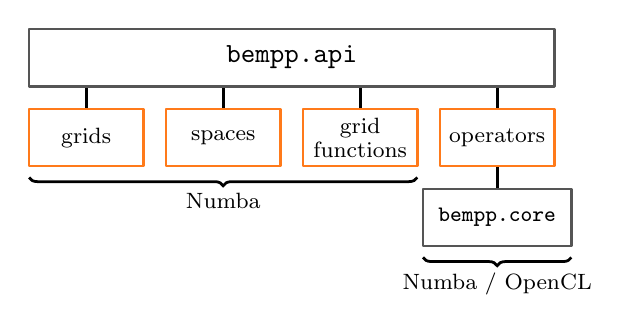
\begin{tikzpicture}[x=1.45cm,y=-1.45cm]

\draw[line width=1pt] (0.5,0.5) -- (0.5,0.7);
\draw[line width=1pt] (1.7,0.5) -- (1.7,0.7);
\draw[line width=1pt] (2.9,0.5) -- (2.9,0.7);
\draw[line width=1pt] (4.1,0.5) -- (4.1,0.7);
\draw[line width=1pt] (4.1,1.2) -- (4.1,1.4);

\draw[line width=1pt,line join=round,line cap=round,bemppgrey] (0,0) rectangle (4.6,0.5);
\node at (2.3,0.25) {\texttt{bempp.api}};
\draw[line width=1pt,line join=round,line cap=round,bempporange] (0,0.7) rectangle (1,1.2);
\node at (0.5,0.95) {\footnotesize grids};
\draw[line width=1pt,line join=round,line cap=round,bempporange] (1.2,0.7) rectangle (2.2,1.2);
\node at (1.7,0.95) {\footnotesize spaces};
\draw[line width=1pt,line join=round,line cap=round,bempporange] (2.4,0.7) rectangle (3.4,1.2);
\node at (2.9,0.95) [text width=1.45cm,align=center] {\footnotesize grid\\[-1.2mm]functions};
\draw[line width=1pt,line join=round,line cap=round,bempporange] (3.6,0.7) rectangle (4.6,1.2);
\node at (4.1,0.95) {\footnotesize operators};
\draw[line width=1pt,line join=round,line cap=round,bemppgrey] (3.45,1.4) rectangle (4.75,1.9);
\node at (4.1,1.65) {\footnotesize\texttt{bempp.core}};

\draw[line width=1pt,decorate,decoration={brace,amplitude=3pt,mirror}] (0,1.3) -- (3.4,1.3);
\node[anchor=north] at (1.7,1.35) {\footnotesize Numba};

\draw[line width=1pt,decorate,decoration={brace,amplitude=3pt,mirror}] (3.45,2) -- (4.75,2);
\node[anchor=north] at (4.1,2.05) {\footnotesize Numba / OpenCL};
\end{tikzpicture}

\section{ASSEMBLING BOUNDARY INTEGRAL OPERATORS WITH OPENCL}

In this section, we discuss in more detail the assembly of boundary integral operators with OpenCL
and how we integrated this into our Python workflow. We start with a brief introduction to OpenCL and then
dive into how we use OpenCL as part of Bempp-cl.

\subsection{What is OpenCL?}

OpenCL \cite{opencl} is a heterogeneous compute standard for CPUs, GPUs, FPGAs, and other types of devices that provide conformant drivers. At its core, OpenCL executes compute kernels that can be written in C99, or (more recently) in C++. The current version of OpenCL is 3.0, though the most widely implemented standard is OpenCL 1.2, which Bempp-cl uses.

OpenCL splits computational tasks into work-items, each of which represents a single execution of a compute kernel. Work items are grouped together into work groups, which share local memory. Barrier synchronization is only allowed within a work group. All work items are uniquely indexed by a one, two, or three dimensional index space, called NDRange. Kernels are launched onto a compute device (e.g., a CPU or GPU) from a host device. OpenCL allows kernels to be loaded as strings and compiled on the fly for a given device, making it well suited for launching from high-productivity languages.

To launch an OpenCL kernel the user must first initialize buffers on the compute device, then copy any relevant data from host to the compute device. A kernel string can then be loaded and just-in-time compiled for the device. The kernel is then run, and the results can be copied back to the host.

OpenCL has very good support for vectorized operations: it provides vector data types and defines a number of standard operations for these vector types. For example, the type \ocl{double4} will allow four double values to be held in a SIMD register. This makes it easy to explicitly target modern SIMD execution in a portable way while avoiding difficult compiler intrinsics and keeping kernel code readable.

Python has excellent OpenCL support through the PyOpenCL library by Andreas Kloeckner \cite{pyopencl}. PyOpenCL automates much of the initialization of the OpenCL environment and makes it easy to create buffers and launch OpenCL kernels from Python.

\subsection{OpenCL Assembly in Bempp-cl}

\begin{figure*}
	\center
	\begin{opencl}
#include "bempp_base_types.h"
#include "bempp_helpers.h"
#include "bempp_spaces.h"
#include "kernels.h"

__kernel void kernel_function(
    __global uint* testIndices, __global uint* trialIndices,
    __global int* testNormalSigns, __global int* trialNormalSigns,
    __global REALTYPE* testGrid, __global REALTYPE* trialGrid,
    __global uint* testConnectivity, __global uint* trialConnectivity,
    __global uint* testLocal2Global, __global uint* trialLocal2Global,
    __global REALTYPE* testLocalMultipliers, __global REALTYPE* trialLocalMultipliers,
    __constant REALTYPE* quadPoints, __constant REALTYPE* quadWeights,
    __global REALTYPE* globalResult,
    __global REALTYPE* kernel_parameters,
    int nTest, int nTrial, char gridsAreDisjoint)
{
  /* */
}
\end{opencl}

	\caption{Definition of the OpenCL compute kernel for scalar integral equations.}
	\label{fig:kernel_definition}
\end{figure*}

Bempp-cl has OpenCL kernels for all its boundary operators. All operators have the same interface and are launched in the same way. In the first step, the relevant data will need to be copied to the compute device. This data consists of:

\begin{itemize}
	\item Test and trial indices of triangles over which to be integrated.
	\item Signs of the normal directions for the spaces.
	\item Test and trial grid as flat floating point array, defining each triangle through nine floating point numbers, specifying the $(x, y, z)$ coordinates of each of the three nodes of a triangle.
	\item Test and trial connectivity information that stores the indices of each node for each triangle.
	\item Test and trial mappings of local triangle degrees of freedom to global degrees of freedom.
	\item Test and trial basis function multipliers for each triangle.
	\item Quadrature points and quadrature weights.
	\item A buffer that contains the global assembled matrix.
	\item Additional kernel parameters, such as the wavenumber for Helmholtz problems.
	\item Number of test and trial degrees of freedom.
	\item A single byte that is set to one if the test and trial grids are disjoint.
\end{itemize}

An example kernel definition is shown in \cref{fig:kernel_definition}.
Before the kernel can be launched, it needs to be configured and just-in-time compiled. Kernel configuration happens through C-style preprocessor definitions that are passed through the just-in-time compiler. These include the names of the test and trial space, the name of the function that evaluates the Green's function, whether we are using single or double precision types, and (for SIMD enhanced kernels) the vector length of the SIMD types.
For example, in \cref{fig:kernel_definition} all floating point types have the name \ocl{REALTYPE}. This is substituted with either \ocl{float} or \ocl{double} during just-in-time compilation.

Each work-item computes (using numerical quadrature) all interactions of basis functions on the trial element with basis functions on the test element. Before summing the result into the global result buffer, the kernel checks via the connectivity information if the test and trial triangles are adjacent or identical (see \cref{fig:triangles}). To do this, it simply checks if at at least one of the node indices of the test triangle is equal to one of the node indices of the trial triangle. If this is true and the grids are not disjoint, the result of the kernel is discarded and not summed back into the global result buffer: for these triangles, separate singular quadrature rules need to be used. The effect is that a few work-items do work that is discarded. However, in a grid with $N$ elements, the number of triangle pairs requiring a singular quadrature rule is $\mathcal{O}(N)$, while the total number of interactions is $N^2$. Hence, only a tiny fraction of work-items are discarded.

\subsection{SIMD optimized kernels}
When we are running on a CPU and want to take advantage of available SIMD optimizations, we need to make a few modifications to our approach. The corresponding kernel works similarly to described above, but we compute a batch of interactions between one test triangle and $X$ trial triangles, where $X$ is either 4, 8, or 16 (depending on the number of available SIMD lanes). This strategy allows us to optimize almost all floating point operations within a kernel run for SIMD operation. If the number of trial elements is not divisible by 4, 8, or 16, then the few remaining trial elements are assembled with the standard-non vectorized kernel.

Each kernel definition is stored in two variants, one with the ending \texttt{\_novec.cl} and another one with the ending \texttt{\_vec.cl}. The vectorized variant is configured via preprocessor directives for the desired number of vector lanes. Having to develop two OpenCL kernel codes for each operator creates a certain amount of overhead, but once we have implemented the non-vectorized version then, with the help of preprocessor directives and a number of helper functions that do the actual implementation of operations depending on whether the kernel is vectorized or not, it is usually only a matter of an hour or two to convert the non-vectorized kernel into a vectorized version.

Alternatively, some CPU OpenCL runtime environments can (optionally) try and auto-vectorize kernels by batching together work items on SIMD lanes, similar to what we do manually. In our experience, this works well for very simple kernels but often fails for more complex OpenCL kernels. This is why we decided to implement this strategy manually.

A completely different SIMD strategy could be taken by batching together quadrature evaluations within a single test/trial pair. There are two disadvantages to this approach: first, it only works well if the number of quadrature points is a multiple of the available SIMD lanes. Second, other operations such as the geometry calculations for each element then cannot be SIMD optimized as these are only performed once per test/trial pair.

\subsection{Assembling the singular part of integral operators}
The assembly of the singular part of an integral operator works a bit differently. Remember that the singular part consists of triangle parts which are adjacent to each other or identical (the three later cases in \cref{fig:triangles}): there are $\mathcal{O}(N)$ such pairs. We are using fully numerical quadrature rules for these integrals that are based on subdividing the four-dimensional integration domain and using transformation techniques to remove the singularities. This gives highly accurate evaluation of these integration pairs but requires a large number (typically over $1000$) quadrature points per triangle pair.

For this assembly, we create one workgroup for each triangle pair. Inside this workgroup, we have a number of work-items that evaluate the quadrature rules then sum up the results. Depending on how two triangles are related to each other, different types of singular quadrature rule are needed. We solve this by pre-loading all possible quadrature rules onto the device, and also store for each triangle pair an index pointing to the required quadrature rule so that the kernel function can select the correct rule to evaluate. For the singular quadrature rules, we did not implement separate SIMD optimized kernels as the proposed implementation is already highly efficient and requires only a fraction of the computational time of the regular quadrature rules described above. At the end, the singular integral values are either summed into the overall result matrix, or (if desired by the user) stored as separate sparse matrix.

\subsection{Avoiding data races in the global assembly}


\section{NUMBA ASSEMBLY OF INTEGRAL OPERATORS}
The main focus of Numba within Bempp-cl is to provide accelerated implementations of routines with linear complexity, such as grid iterations, integration of functions over grids, or assembly of certain sparse matrices. However, we also provide a fall-back implementation of the OpenCL dense operator assembly in Numba.

With Numba, we use classic loop parallelism: each loop iteration is the assembly of one test element with all trial elements. Within each loop we try to optimize for auto-vectorization by linearly passing through the data in memory order for the individual operations. However, a much smaller fraction of operations is SIMD optimized due to the lack of targeted SIMD constructs in Numba.

\section{PERFORMANCE BENCHMARKS}

In this section we want to provide a number of performance benchmarks. The tests are running on an Intel i9-9980HK with a base clock of 2.4GHz and a burst clock of 5GHz. The CPU supports AVX, AVX2, and AVX-512.
The tests are running on a Dell Precision 7740 Workstation Laptop, meaning the burst clock can not be maintained due to cooling. As GPU we use an Nvidia RTX 3000 GPU. All benchmarks are running within Linux. For OpenCL on the GPU we use the Nvidia GPU drivers and as CPU runtime we compare the open-source POCL driver against the Intel CPU OpenCL runtime environment.

\subsection{Benchmarking a simple Laplace single-layer boundary operator}

\subsection{Complex arithmetic benchmark - A Helmholtz Kernel}

\subsection{CPU vs GPU for evaluating domain potential operators}


\subsection{Solving a complete electromagnetic problem}




\bibliographystyle{IEEEtran}
\begin{thebibliography}{1}

\bibitem{Bempp-cl}
T. Betcke and M. W. Scroggs,
``Bempp-cl: A fast Python based just-in-time compiling boundary element library,''
{\it Journal of Open Source Software}, vol. 6, no. 59, p. 2879, 2021.
\textsc{doi}: \href{https://dx.doi.org/10.21105/joss.02879}{10.21105/joss.02879}.

\bibitem{erichsen}
S. Erichsen, and A. Sauter,
``Efficient automatic quadrature in 3-d Galerkin BEM,''
{\it Computer Methods in Applied Mechanics and Engineering}, vol. 157, no. 3, pp. 215--224, 1998.
\textsc{doi}: \href{https://doi.org/10.1016/S0045-7825(97)00236-3}{10.1016/S0045-7825(97)00236-3}.

\bibitem{pyopencl}
A. Kloeckner, N. Pinto, Y. Lee, B. Catanzaro, P. Ivanov, and A. Fasih,
``PyCUDA and PyOpenCL: A scripting-based approach to GPU run-time code generation,''
{\it Parallel Computing}, vol. 38, no. 3, pp. 157--174, 2012.
\textsc{doi}: \href{https://dx.doi.org/10.1016/j.parco.2011.09.001}{10.1016/j.parco.2011.09.001}.



\bibitem{opencl}
OpenCL, \url{https://www.khronos.org/opencl/}.


\bibitem{bempp_maxwell}
M. W. Scroggs, T. Betcke, E. Burman, Wojciech \'{S}migaj, and E. van 't Wout, ``Software frameworks for integral equations in electromagnetic scattering based on Cader\'{o}n identities''
{\it Computers \& Mathematics with Applications}, vol. 74, no. 11, pp. 2897--2914, 2017.
\textsc{doi}: \href{https://doi.org/10.1016/j.camwa.2017.07.049}{10.1016/j.camwa.2017.07.049}.

\bibitem{bempp_orig}
W. \'{S}migaj, T. Betcke, S. Arridge, J. Phillips, and M. Schweiger,
``Solving boundary integral problems with BEM++,''
{\it ADM Transactions on Mathematical Software}, vol. 41, no. 2, article 6, 2015.
\textsc{doi}: \href{https://doi.org/10.1145/2590830}{10.1145/2590830}
	
\bibitem{bempp_exafmm}
T. Wang, C. D. Cooper, T. Betcke, and L. A. Barba,
``High-productivity, high-performance workflow for virus-scale electrostatic simulations with Bempp-ExaFMM,''
2021.
arXiv (preprint): \href{https://arxiv.org/abs/2103.01048}{2103.01048}.
\end{thebibliography}

\end{document}
